% !TEX TS-program = xelatex
% !TEX encoding = UTF-8 Unicode
% !Mode:: "TeX:UTF-8"
\documentclass{resume}
%\documentclass[8pt]{article}
%\usepackage{zh_CN-Adobefonts_external} % Simplified Chinese Support using external fonts (./fonts/zh_CN-Adobe/)
\usepackage{zh_CN-Adobefonts_internal} % Simplified Chinese Support using system fonts
\usepackage{linespacing_fix} % disable extra space before next section
\usepackage{cite}
\usepackage[colorlinks,linkcolor=blue,anchorcolor=blue,citecolor=green,urlcolor=blue]{hyperref}
\usepackage{amssymb}
\usepackage{amsmath}


%for header image
\usepackage{graphicx}
\usepackage{tikz} %用于定位照片
\usetikzlibrary{calc}
%for floating figures
\usepackage{wrapfig}
\usepackage{float}
%\floatstyle{boxed}
%\restylefloat{figure}


\newcommand{\vcenteredinclude}[1]{\begingroup
\setbox0=\hbox{\hspace*{-2.9cm}\includegraphics[width=1.2cm]{#1}}%
\parbox{\wd0}{\box0}\endgroup}


\begin{document}
\pagenumbering{gobble} % suppress displaying page number

\name{ 张\hspace{0.1cm}贵\hspace{0.1cm}瑞 }

% {E-mail}{mobilephone}{homepage}
% be careful of _ in emaill address
{\centerline{\contactInfo{17781444956@163.com}{177-8144-4956}{1997-02-23}}}
{\centerline{GitHub:\hyperlink{https://github.com/freesix}{https://github.com/freesix}}}
\begin{tikzpicture}[remember picture,overlay]
  \node[anchor = north east] at ($(current page.north east)+(-2cm,-1.2cm)$){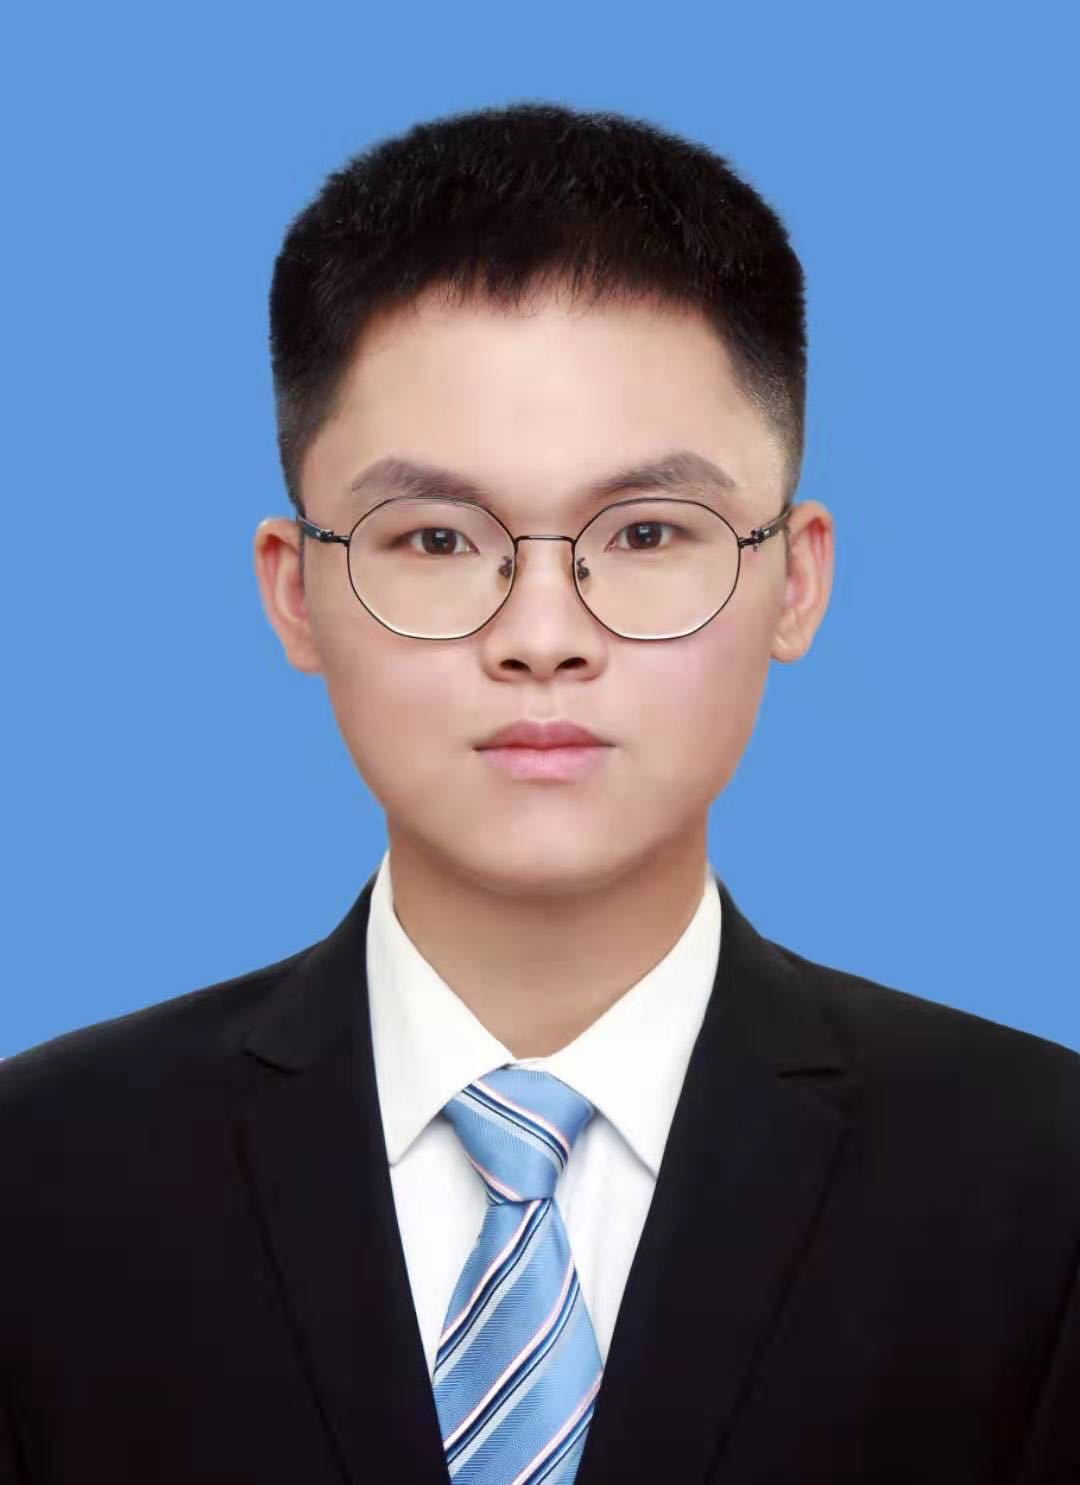
\includegraphics[width=2.5cm]{images/照片.jpg}};
\end{tikzpicture}
% \centerline{\includegraphics[width=0.2cm]{imazhen.jpg}}

% {E-mail}{mobilephone}
% keep the last empty braces!
%\contactInfo{xxx@yuanbin.me}{(+86) 131-221-87xxx}{}



\section{\faGraduationCap 教育工作背景}

\datedsubsection{\textbf{西南民族大学}, 电气工程学院}{2021年9月 -- 2024年6月}
\textit{硕士}\ \ 电子信息专业

\datedsubsection{\textbf{上海芯圣电子股份有限公司}}{2020年5月 -- 2021年8月}
\textit{FAE工程师}

\datedsubsection{\textbf{上海工程技术大学}, 电气工程学院}{2016年9月 -- 2020年7月}
\textit{学士}\ \ 自动化专业


\section{\faCogs\ 技能}
% increase linespacing [parsep=0.5ex]
\begin{itemize}[parsep=0.5ex]
  \item 熟悉Python、C、C++、LaTex、Matlab、Linux
  \item 对图像拼接有一定了解,有在研项目支持
  \item 对图神经网络和图匹配相关算法有一定了解
  \item 了解李群李代数、对极几何、图优化等,对相应算法库Eigen、g2o、OpenCV等有一定使用
  \item 了解ORB\_SLAM3、Point-LIO框架
\end{itemize}


\section{\faUsers\ 科研 / 项目经历}

\datedsubsection{\textbf{便携式血氧仪算法和硬件改进}}{2020年7月 -- 2021年8月}
\begin{itemize}
\item  提升血氧仪在不同测量状况下的测量准确率。对剧烈运动、手指放置不正确等异常增加修改相应程序
\item  主控芯片的改版,重新设计PCB以降低硬件成本
\end{itemize}

\datedsubsection{\textbf{多曲面图像拼接补全算法设计}}{2022年12月 -- 至今}
\begin{itemize}
\item  根据横向项目的需求制定技术路线,撰写需求分析、技术目标等文档
\item  对项目中图像的畸变、失焦、配准、像素缺失等关键问题提出技术路线
\item  提出了一种权重可学习的图注意力机制用于图像拼接的配准步骤,性能优于SuperGlue
\end{itemize}

\datedsubsection{\textbf{锂电充手电开发}}{2020年12月 -- 2021年8月}
\begin{itemize}
  \item 负责整体项目评估和框架搭建
  \item 编写功能模块代码
\end{itemize}

\datedsubsection{\textbf{新东方七宝校区营销负责人(实习)}}{2018年5月 -- 2019年1月}
\begin{itemize}
  \item 制定地推策略、选取发放物料、人员招聘、点位选取、人员考勤监督等
\end{itemize}


\section{\faPaperPlane\ 获奖和科研成果}
\hspace*{0.8cm}
\begin{itemize}
  \item $\ll$ Image Stitching with Weight Learnable Graph Matching Network$\gg$ (暂定),已完成模型的训练,尚在验证与讨论阶段
  \item 研究生奖学金两次
  \item 本科生奖学金一次
  \item 本科校三等奖一次
\end{itemize}



%% Reference
%\newpage
%\bibliographystyle{IEEETran}
%\bibliography{mycite}
\end{document}
